%%%%%%%%%%%%%%%%%%%%%%%%%%%%%%%%%%%%%%%%%
% Beamer Presentation
% LaTeX Template
% Version 1.0 (10/11/12)
%
% This template has been downloaded from:
% http://www.LaTeXTemplates.com
%
% License:
% CC BY-NC-SA 3.0 (http://creativecommons.org/licenses/by-nc-sa/3.0/)
%
%%%%%%%%%%%%%%%%%%%%%%%%%%%%%%%%%%%%%%%%%

%----------------------------------------------------------------------------------------
%	PACKAGES AND THEMES
%----------------------------------------------------------------------------------------

\documentclass[UTF8,aspectratio=169,12pt]{ctexbeamer}

\usepackage{hyperref}
\hypersetup{
	colorlinks=true,
	linkcolor=red,
	anchorcolor=blue,
	citecolor=green
}

\mode<presentation> {
	
	% The Beamer class comes with a number of default slide themes
	% which change the colors and layouts of slides. Below this is a list
	% of all the themes, uncomment each in turn to see what they look like.
	
	%\usetheme{default}
	%\usetheme{AnnArbor}
	%\usetheme{Antibes}
	%\usetheme{Bergen}
	%\usetheme{Berkeley}
	%\usetheme{Berlin}
	%\usetheme{Boadilla}
	%\usetheme{CambridgeUS}
	%\usetheme{Copenhagen}
	%\usetheme{Darmstadt}
	%\usetheme{Dresden}
	%\usetheme{Frankfurt}
	%\usetheme{Goettingen}
	%\usetheme{Hannover}
	%\usetheme{Ilmenau}
	%\usetheme{JuanLesPins}
	%\usetheme{Luebeck}
	\usetheme{Madrid}
	%\usetheme{Malmoe}
	%\usetheme{Marburg}
	%\usetheme{Montpellier}
	%\usetheme{PaloAlto}
	%\usetheme{Pittsburgh}
	%\usetheme{Rochester}
	%\usetheme{Singapore}
	%\usetheme{Szeged}
	%\usetheme{Warsaw}
	
	% As well as themes, the Beamer class has a number of color themes
	% for any slide theme. Uncomment each of these in turn to see how it
	% changes the colors of your current slide theme.
	
	%\usecolortheme{albatross}
	%\usecolortheme{beaver}
	%\usecolortheme{beetle}
	%\usecolortheme{crane}
	%\usecolortheme{dolphin}
	%\usecolortheme{dove}
	%\usecolortheme{fly}
	%\usecolortheme{lily}
	%\usecolortheme{orchid}
	%\usecolortheme{rose}
	%\usecolortheme{seagull}
	%\usecolortheme{seahorse}
	%\usecolortheme{whale}
	%\usecolortheme{wolverine}
	
	%\setbeamertemplate{footline} % To remove the footer line in all slides uncomment this line
	%\setbeamertemplate{footline}[page number] % To replace the footer line in all slides with a simple slide count uncomment this line
	
	%\setbeamertemplate{navigation symbols}{} % To remove the navigation symbols from the bottom of all slides uncomment this line
}

\usepackage{graphicx} % Allows including images
\graphicspath{{./figs/}}
\usepackage{booktabs} % Allows the use of \toprule, \midrule and \bottomrule in tables
\usepackage{longtable}
\usepackage{xcolor}
\usepackage{minted}
\usepackage{listings}
\lstset{numbers=left, %设置行号位置
	numberstyle=\tiny, %设置行号大小
	keywordstyle=\color{blue}, %设置关键字颜色
	commentstyle=\color[cmyk]{1,0,1,0}, %设置注释颜色
	frame=single, %设置边框格式
	escapeinside=``, %逃逸字符(1左面的键),用于显示中文
	%breaklines, %自动折行
	extendedchars=false, %解决代码跨页时,章节标题,页眉等汉字不显示的问题
	xleftmargin=2em,xrightmargin=2em, aboveskip=1em, %设置边距
	tabsize=4, %设置tab空格数
	showspaces=false %不显示空格
}
% Fonts
% \usepackage{libertine}
% \setmonofont{Courier}
%\setCJKsansfont[ItalicFont=Noto Serif CJK SC Black, BoldFont=Noto Sans CJK SC Black]{Noto Sans CJK SC}


%----------------------------------------------------------------------------------------
%   TITLE PAGE
%----------------------------------------------------------------------------------------

\title[第4讲]{第四讲:存储管理} % The short title appears at the bottom of every slide, the full title is only on the title page
\subtitle{第7节:ch6 - 文件系统}
\author{向勇、陈渝、李国良} % Your name
\institute[清华大学] % Your institution as it will appear on the bottom of every slide, may be shorthand to save space
{
清华大学计算机系 \\ % Your institution for the title page
\medskip
\textit{xyong,yuchen,liguoliang@tsinghua.edu.cn} % Your email address
}
\date{\today} % Date, can be changed to a custom date

\begin{document}

\begin{frame}
\titlepage % Print the title page as the first slide
\end{frame}

%----------------------------------------------------------------------------------------
%\begin{frame}
%\frametitle{提纲} % Table of contents slide, comment this block out to remove it
%\tableofcontents % Throughout your presentation, if you choose to use \section{} and \subsection{} commands, these will automatically be printed on this slide as an overview of your presentation
%\end{frame}

%----------------------------------------------------------------------------------------
%   PRESENTATION SLIDES
%----------------------------------------------------------------------------------------
%------------------------------------------------
\section{第7节:ch6 - 文件系统}% Sections can be created in order to organize your presentation into discrete blocks, all sections and subsections are automatically printed in the table of contents as an overview of the talk
%------------------------------------------------
%\subsection{页表数据结构}
% 
% #### 7. 实验六:文件系统
% 
%------------------------------------------------
\begin{frame}
	\frametitle{文件接口}
% %%%%%%  文件接口
% 
		\begin{itemize}
		\item \href{https://rcore-os.github.io/rCore-Tutorial-Book-v3/chapter6/1file-descriptor.html\#id3}{文件}:所有输入输出都被视为文件操作(Everything is a file)
		\item 统一的 `File`抽象\href{https://github.com/rcore-os/rCore-Tutorial-v3/blob/ch6/os/src/fs/mod.rs\#L5}{接口}
		\end{itemize}
    \begin{figure}
        \centering
        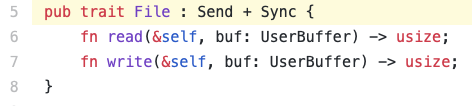
\includegraphics[width=0.6\linewidth]{lecture04/figs/mod-L5.png}
%       \caption{xxxx}
    \end{figure}
% 
% [mod-L5](/Users/xyong/github/os-lectures/lecture04/figs/mod-L5.png)
% 
		\begin{itemize}
		\item 用户缓冲区的抽象 `UserBuffer`:\href{https://github.com/rcore-os/rCore-Tutorial-v3/blob/ch6/os/src/mm/page_table.rs\#L199}{struct UserBuffer}
		\end{itemize}
    \begin{figure}
        \centering
        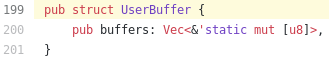
\includegraphics[width=0.6\linewidth]{figs/page_table-L199.png}
%       \caption{xxxx}
    \end{figure}
% 
% [page_table-L199](/Users/xyong/github/os-lectures/lecture04/figs/page_table-L199.png)
% 
\end{frame}
%------------------------------------------------
\begin{frame}
	\frametitle{标准输入和输出文件实现}
% %%%%%%  标准输入和输出文件实现
% 
% \href{https://rcore-os.github.io/rCore-Tutorial-Book-v3/chapter6/1file-descriptor.html\#id3}{标准输入和标准输出}
% 
标准输入:\href{https://github.com/rcore-os/rCore-Tutorial-v3/blob/ch6/os/src/fs/stdio.rs\#L10}{stdin}
    \begin{figure}
        \centering
        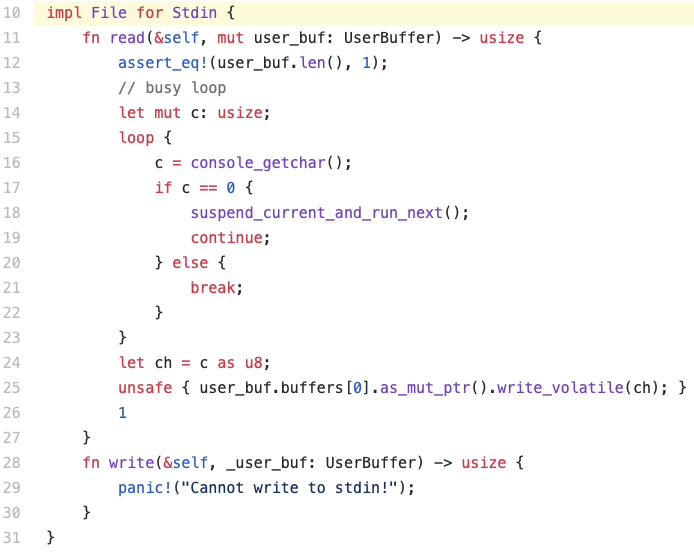
\includegraphics[width=0.6\linewidth]{figs/stdio-L10.png}
%       \caption{xxxx}
    \end{figure}
% 
% [stdio-L10](/Users/xyong/github/os-lectures/lecture04/figs/stdio-L10.png)
% 
\end{frame}
%------------------------------------------------
\begin{frame}
	\frametitle{标准输入和输出文件实现}
标准输出:\href{https://github.com/rcore-os/rCore-Tutorial-v3/blob/ch6/os/src/fs/stdio.rs\#L33}{stdout}
    \begin{figure}
        \centering
        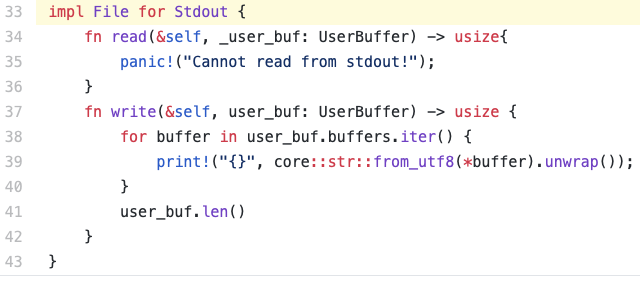
\includegraphics[width=0.6\linewidth]{figs/stdio-L33.png}
%       \caption{xxxx}
    \end{figure}
% 
% [stdio-L33](/Users/xyong/github/os-lectures/lecture04/figs/stdio-L33.png)
% 
\end{frame}
%------------------------------------------------
\begin{frame}
	\frametitle{\href{https://rcore-os.github.io/rCore-Tutorial-Book-v3/chapter6/1file-descriptor.html\#id5}{文件描述符与文件描述符表}}
% %%%%%%  文件描述符
% 
进程控制块中的文件描述符表、进程的标准输入输出
    \begin{figure}
        \centering
        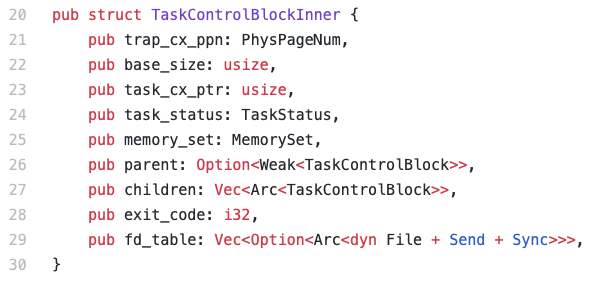
\includegraphics[width=0.6\linewidth]{figs/task-L20.png}
%       \caption{xxxx}
    \end{figure}
% 
% [task-L20](/Users/xyong/github/os-lectures/lecture04/figs/task-L20.png)
% 
% \href{https://github.com/rcore-os/rCore-Tutorial-v3/blob/ch6/os/src/task/task.rs\#L20}{进程控制块中的文件描述符表}:在进程创建时,缺省打开标准输入和输出;
% 
\end{frame}
%------------------------------------------------
\begin{frame}
	\frametitle{\href{https://rcore-os.github.io/rCore-Tutorial-Book-v3/chapter6/1file-descriptor.html\#id6}{文件读写系统调用}}
% %%%%%%  文件相关的系统调用
% 
基于文件抽象接口和文件描述符表,可以让文件读写系统调用 sys\_read/write 变得更加通用;
    \begin{figure}
        \centering
        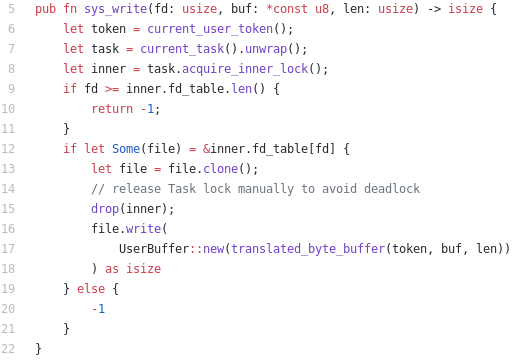
\includegraphics[width=0.6\linewidth]{figs/fs-L5.png}
%       \caption{xxxx}
    \end{figure}
% 
% [fs-L5](/Users/xyong/github/os-lectures/lecture04/figs/fs-L5.png)

% 
\end{frame}
%----------------------------------------------------------------------------------------

\end{document}
